% THIS IS A LATEX TEMPLATE FILE FOR PAPERS INCLUDED IN THE
% *Anthology of Computers and the Humanities*. ADD THE OPTION
% 'final' WHEN CREATING THE FINAL VERSION OF THE PAPER. 
% DO NOT change the documentclass
%\documentclass[final]{anthology-ch} % for the final version
\documentclass[final]{anthology-ch}         % for the submission

% LOAD LaTeX PACKAGES
\usepackage{booktabs}
\usepackage{float}
\usepackage{subfig}
\usepackage{graphicx}
\usepackage{wrapfig}
\usepackage{verbatim}
\usepackage[export]{adjustbox}
\usepackage{svg}
%\usepackage{framed}
% ADD your own packages using \usepackage{}
\usepackage{fontspec}
\setmainfont{Tinos}

% TITLE OF THE SUBMISSION
% Change this to the name of your submission
\title{Castles, Battlefields, and Continents: A Dataset of Maps from Literature}

% AUTHOR AND AFFILIATION INFORMATION
% For each author, include a new call to the \author command, with
% the numbers in brackets indicating the associated affiliations 
% (next section) and ORCID-ID for each author.  
\author[1]{Axel Bax}[
  orcid=0009-0001-4728-1909
]

\author[1]{David Mimno}[
  orcid=0000-0001-7510-9404
]

% While we encourage including ORCID-IDs for all authors, you can
% include authors that do not have one by definining an empty ID.
\author[1]{Matthew Wilkens}[
  orcid=0000-0001-6749-9318
]

% There should be one call to \affiliation for each affiliation of
% the authors. Multiple affiliations can be given to each author
% and an affiliation can be given to multiple authors. 
\affiliation{1}{Information Science, Cornell University, Ithaca, New York}

% KEYWORDS
% Provide one or more keywords or key phrases seperated by commas
% using the following command
\keywords{computational humanities, literary cartography, digital humanities, CLIP, EfficientNet, maps}

% METADATA FOR THE PUBLICATION
% This will be filled in when the document is published; the values can
% be kept as their defaults when the file is submitted
\pubyear{2025}
\pubvolume{3}
\pagestart{280}
\pageend{280}
\conferencename{Computational Humanities Research 2025}
\conferenceeditors{Taylor Arnold, Margherita Fantoli, and Ruben Ros}
\doi{10.63744/oYbvYsUA743D}  
\paperorder{19} 

\addbibresource{bibliography.bib}

%%%%%%%%%%%%%%%%%%%%%%%%%%%%%%%%%%%%%%%%%%%%%%%%%%%%%%%%%%%%%%%%%%%%%%%%%%%
% HERE IS THE START OF THE TEXT
\begin{document}

\maketitle

\begin{abstract}

\noindent Maps are not common in novels. It is not obvious that they are necessary at all. Yet maps do appear in some novels. Why and to what ends? To answer these questions, scholars need a large collection of novels that contain maps. We develop a computational system to identify maps from page images and apply it to a large historical corpus of fiction. We deploy a three part workflow using an ensemble of three finetuned EfficientNet convolutional neural network (CNN) classifiers, Contrastive Language-Image Pre-training (CLIP), and human annotation to identify 2,622 maps in over 32 million pages of fiction published 1800--1928. We find that 1) maps are rare, making up 0.008\% of all pages (1.7\% of novels contain at least one map) 2) ``map novels'' were most common at the turn of the 20th century, 3) maps mostly appear on endpapers or front matter, 4) only 43\% of map novels contain references to maps in their library MARC records, 5) 25\% of maps depict fictional settings, 6) 70\% of maps represent areas at a regional or larger scale, and 7) map novels contain more spatial language than non-map novels.
\end{abstract}

\section{Introduction} 

When asked about novels that contain maps, nearly every reader can think of an example. But not all novels contain maps; in fact, most do not. There is no obvious rule that dictates when a novel should contain a map. Literary cartographers have offered different explanations for why maps appear, and for the historical periods in which maps became more (or less) common. Hegglund and Bushell suggest that maps support the reader's understanding of spatial relationships within the novel~\cite{hegglund2012world,bushell2020reading}. Alternatively, maps may be aesthetic embellishments, or they may be conventional elements of certain literary genres. Such maps may reflect the capabilities and economic priorities of publishers, rather than the desire of authors. 

Each of these claims has potential merit. But to address any of them, we must first develop methods to identify maps in large collections of novels. Identifying as many \emph{novel maps} (i.e., maps that appear in narrative fiction) as possible will allow us to characterize the contexts in which maps appear and to generalize about the content of both novel maps and \emph{map novels} (novels that contain maps). In this paper, we present such a system, along with a preliminary analysis of thousands of identified maps in nearly 100,000 volumes of English-language fiction.\footnote{The dataset and relevant code can be found at https://github.com/xablexa/maps-from-fiction} We find that 1) maps are exceedingly rare within fiction, making up 0.008\% of all pages; map novels make up just 1.7\% of all novels, 2) map novels were most popular at the turn of the 20th century, 3) maps mostly appear on endpapers or front matter, 4) only 43\% of map novels contain references to maps in their library MARC record, 5) 25\% of maps depict fictional settings and 75\% depict real settings, 6) 71\% of maps represent areas at a regional scale, 21\% at a city scale, and 8\% at an estate scale, and 7) map novels contain more spatial language than non-map novels, especially geospatial prepositions and generic locations.

Maps are relatively easy for humans to identify, but the content of maps (e.g., lots of squiggly lines) can be similar to illustrations that also appear in novels, which makes it difficult to train effective cartographic image classification models. This problem can be addressed via human inspection, but the scale of literary history renders a purely human detection pipeline untenable. Additionally, the goal of identifying \emph{every} map requires a more careful approach than one that simply optimizes accuracy.


\section{Related Work}
Literary cartography projects have especially benefited from computational approaches, as geographic information systems (GIS) have made it much easier to create accurate maps of literary settings and events. Often, these analyses focus on a specific region, such as Donaldson et al.'s Lake District project~\cite{donaldson2017locating}, or Piatti's \emph{Die Geographie der Literatur}, which focuses on Switzerland~\cite{piatti2008geographie}. Both of these projects use close-reading approaches to identify exactly those places that are referenced within a story, then use GIS and computation to share the results of close reading. However, this form of literary cartography uses maps as a medium for sharing spatial information about a story; they are essentially visualizing the descriptive, geospatial text found in their novels of interest. The bottleneck of this approach is the number of novels that can be closely read by trained scholars.

Other computational scholars have addressed this issue of scale by using various natural language processing (NLP) techniques. Soni et al. develop a fine-tuned large language model (LLM) system to identify character-location coreferences, which they then use to track the order of locations that a character occupies~\cite{soni2023grounding}. Wilkens et al. build on this by using GIS to calculate the actual distances traveled by characters to track protagonist mobility~\cite{wilkens2024small}. This approach uses fictional novels with \emph{nonfictional} settings, as the locations must be geolocatable to a specific coordinate on Earth, which eliminates fictional settings that would register incorrectly or fail to register when location names are matched against a gazetteer. As this process is automated, they can map out the mobility of characters at scale, overcoming the bottleneck of close-reading. While this use of computation builds upon the tradition of literary cartographic scholarship to expand its applications, it fails to capture the mobility trends of fictional settings. This is a difficult task, as names of fictional places can be unique to each novel, some novels contain a mix of fictional and real places, and even if all places could be identified in the text, there is no way to calculate the distances between these locations, as there is no ground truth to relate them to each other.

Both the close reading and existing computational approaches extract spatial information from text alone. Some novels contain maps, which are explicitly geospatial in nature and directly relate to the text. These maps provide precise spatial relationships for locations within a novel, which may be fictional or different from modern maps (as in the case of historic cities). Therefore, integrating a visual spatial element with a textual spatial element will reveal more detailed information about the spatial relationships of places within a novel.

The integration of maps with text implies a multi-modal approach, which has been performed in the context of historical map collections. Mahowald \& Lee ~\cite{mahowald2024integrating} use Contrastive Language-Image Pre-training (CLIP) for querying historical map collections with both text and images. CLIP converts text and images to the same vector space, which makes it useful for image classification tasks with text prompts. Since CLIP has been trained on 400 million image-text pairs, it can be applied to different tasks, even without finetuning~\cite{radford2021learning}. Hosseini et al. developed MapReader, an open-source Python library that can be used to query specific map features~\cite{hosseini2022mapreader}. This project uses patches of maps to train for feature classification. These projects provide methodological foundation for classification tasks involving digital maps, but they are focused on existing cartographic collections, rather than extracting maps from another source.

The current project aims to create a collection of maps that appear in novels. This task has long been imagined: John George Bartholomew published his \emph{Literary and Historical Atlas of Europe} in 1910, with the same goal of visualizing the spaces traversed in novels, with both fictional and real settings~\cite{bartholomew1910literary}. In 1999, Moretti created the \emph{Atlas of the European Novel: 1800--1900}, which features a variety of famous maps from literature~\cite{moretti1999atlas}. This atlas is not comprehensive, focusing on maps from Europe in the 19th century, and especially on famous novels. Both of these projects are valuable but biased collections of maps, as they are limited to novels that are well-known, are regional in nature, that relate to the same literary author, or are within a single scholar's area of specialization, making it harder to generalize their collections to broader literary tradition. Like Donaldson et al. and Piatti, these collections are also limited by the number of novels that scholars can read.

\section{Methods}
We seek to identify all maps included in all volumes of English-language fiction, subject to a set of important practical constraints. We begin with 200,000 volumes of fiction held by the HathiTrust digital library as identified in the NovelTM dataset~\cite{underwood2020noveltm}. Because the fiction labeling pipeline for the source dataset was automated, there are some duplicate and nonfiction volumes in the dataset. We removed volumes that were calculated to be $<70\%$ likely to be fiction, though this amounted to only $12\%$ of the dataset.

\begin{wrapfigure}{r}{0.5\textwidth}
    \centering
    %\includesvg[width=\linewidth]{images/FINAL_year_hist_total.svg}
    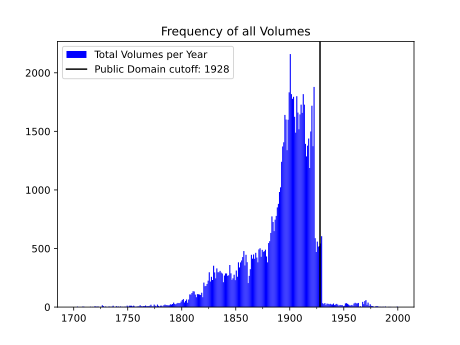
\includegraphics[width=\linewidth]{images/FINAL_year_hist_total.png}
    \caption{Number of novels published per year in the dataset. 1928 denotes the cutoff for public domain in 2024, when this dataset was requested.}
    \label{fig:freq_over_time}
\end{wrapfigure}

The HathiTrust Research Center~\cite{hathitrust} provided data for the 89,914 of these volumes that are in the public domain under US law. These contained individual page scans, individual page text, and volume MARC record information. Images were provided as a mix of TIFF and JPEG2000 files. Among the 89,914 volumes, there are 32,177,400 pages total. These volumes are: likely to be fiction, published 1700--1928,\footnote{There are some novels in the corpus that are in the public domain, but published after 1928. These can give insight into trends after 1928, but are not a representative sample, since they qualify for public domain for reasons other than age.} are written in English, and are in the public domain.

As we are trying to create as close to a comprehensive dataset as possible, we do not want to miss any maps when classifying page scans. This means that an approach prioritizing recall is preferable to one that maximizes accuracy, as is the case in many image classification tasks. Because maps are rare, a highly accurate map classification model could achieve over $99\%$ accuracy by classifying every page as a non-map. Placing value on recall means that we will have many false positives (non-maps classified as maps), but very few false negatives (maps classified as non-maps and thus excluded from the dataset). We implement a multi-stage classification process that values both accuracy and recall, in which we filter our dataset into successively smaller subsets by first removing page scans with very high predicted probabilities of being non-maps, then applying a more expensive model for the next stage. 

We implement 3 stages to our classification process:
\begin{enumerate}
  \item An ensemble of EfficientNet convolutional neural network (CNN) models at different model and image sizes (primary classification).
  \item CLIP, prompted with qualities of maps and non-maps to guide classification (secondary classification).
  \item Manual annotation performed by a human with specific criteria defining maps compared to map-adjacent images (human annotation).
\end{enumerate}

See figure \ref{fig:classifying_workflow} for the entire workflow and number of page scans at each stage.

%\begin{figure}
\begin{wrapfigure}{r}{0.5\textwidth}
\centering
    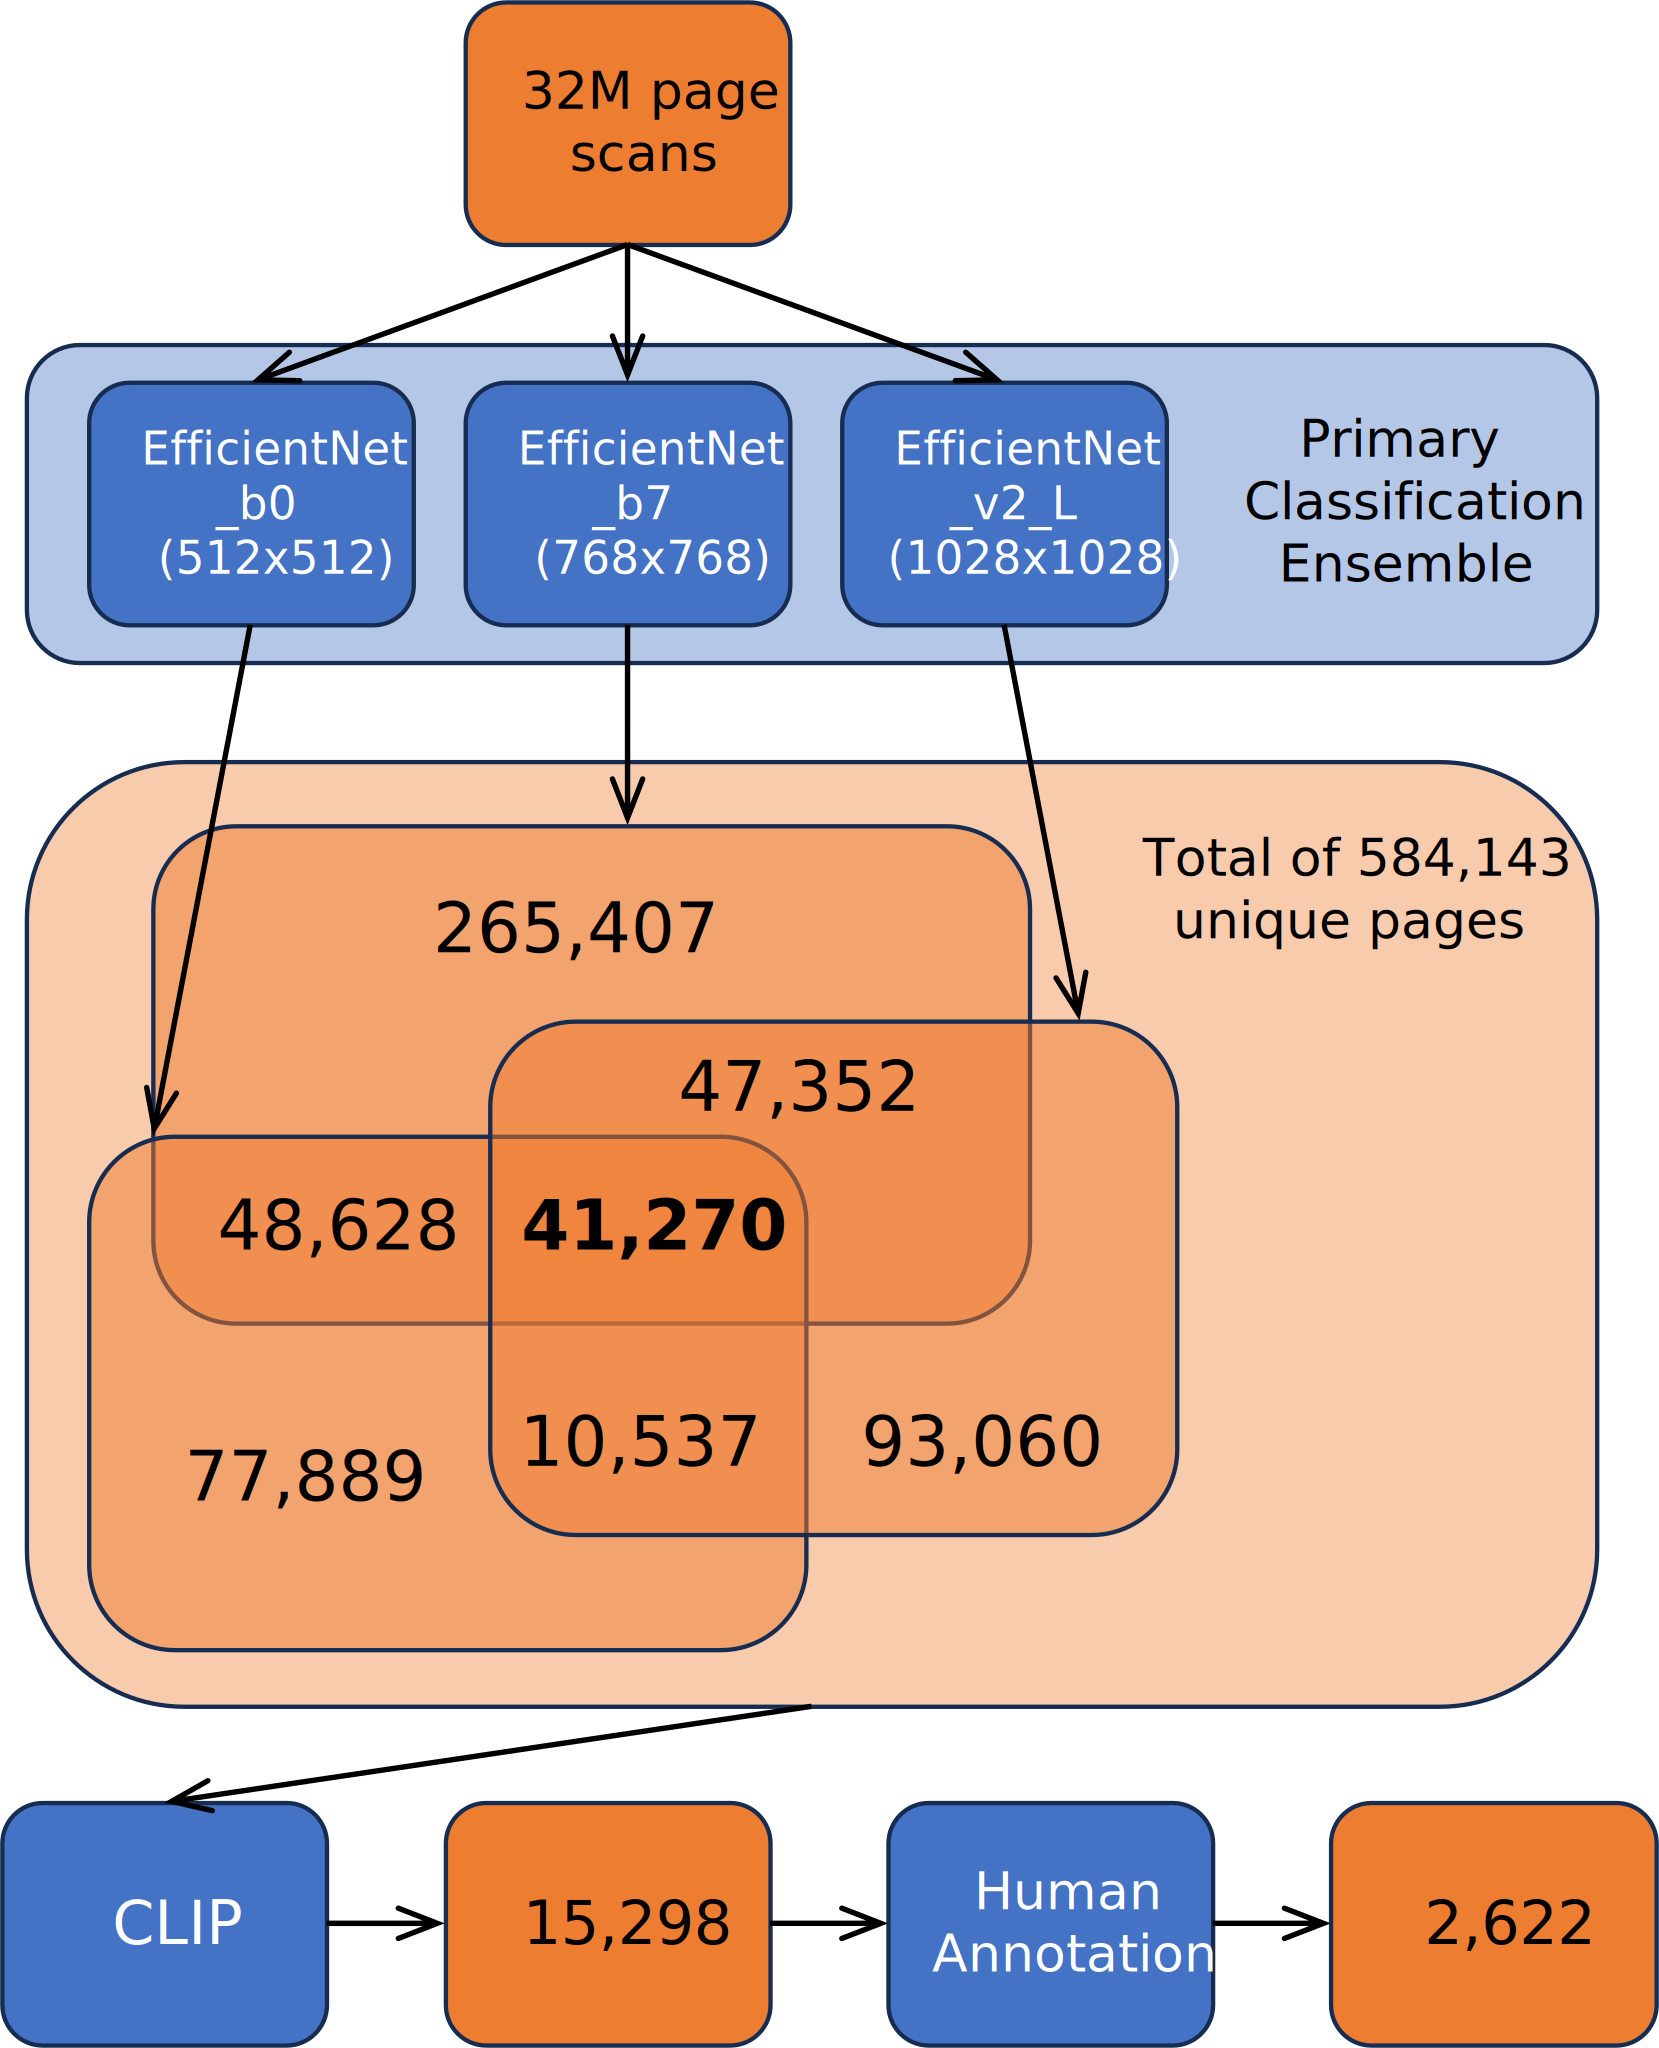
\includegraphics[width=\linewidth]{images/workflow_v3.png}
    \caption{Workflow for identifying maps among page scans. The ensemble processed 32M pages, identifying 584k as maps. CLIP processed these, identifying 15k as maps. We manually examined these, identifying 2,622 maps from 1,557 volumes, the final dataset.}
    \label{fig:classifying_workflow}
\end{wrapfigure}
%\end{figure}

\subsection{Primary Classification}
For the first classification step, we used the EfficientNet CNN, which has been pretrained on over a million images with a thousand object classes~\cite{tan2019efficientnet}. CNNs can be finetuned for a specific task by learning from a set of training images, which makes them useful for this task, as maps that appear in novels are a sufficiently specific concept that they are not among the pretrained ImageNet classes.

Maps are a visually complex concept that changes depending on the region depicted and the style of the cartographer. Therefore, it may be difficult for a CNN to pick out a specific feature that implies that a page scan is a map, rather than, say, an illustration. For this reason, multiple model sizes might identify different combinations of features that suggest an image belongs to the `map' class. Additionally, page scans appear at a variety of sizes, requiring us to downsample scans to a standard size for processing. Downsampling improves processing speed, but reduces the number of pixels in the image, which can make subtler features harder to recognize. For these reasons, we decided to use an ensemble approach -- as multiple model sizes and multiple image sizes might make certain features more or less identifiable as maps -- with the goal of missing as few maps as possible during classification.

We created a finetuning dataset by selecting maps from nonfiction volumes within the same time span as the HathiTrust dataset (1700--1928). This dataset was composed of 730 maps and 270 non-maps, with an 80/20 train/test split. Because maps in fiction are so rare relative to those in nonfiction, it was much easier to gather a training set of images from nonfiction. In doing this, we assume that the general features of maps in nonfiction are similar to those in fiction within the same collection and time period. We duplicated training images with a combination of inversion, rotation, gaussian noise, and magnified patches to maximize the utility of the dataset, as  such resampling has been shown to improve model performance~\cite{kumar2025enhancing}. We optimized all models in the workflow for accuracy first, then, for each model/image size, we chose the model with the highest recall among the top performing models to select the final three models for the ensemble. 

\begin{table}[htb]
\centering
\begin{tabular}{ lr|rrrr }
%\centering
 %\hline
 Model & Image Size & Accuracy & Recall &Precision & $F_1$ \\
 \hline
 EfficientNet\_b0 & 512 & 0.965 & 0.960 & 0.906 & 0.932 \\
 EfficientNet\_b7 & 768 & 0.965 & 0.960 & 0.906 & 0.932 \\
 EfficientNet\_V2\_l & 1024 & 0.970 & 0.961 & 0.925 & 0.942 \\ 
 %\hline
\end{tabular}
\caption{\label{tab:efnet}Evaluation metrics for each classifier in the ensemble. Models were finetuned, then, among the models with the highest accuracy, the one with the highest recall was chosen for each model size. If there was a tie, models that misclassified different maps were prioritized.}
  \label{false_negatives}
\end{table}

We finetuned three image classifiers on this training data to create an ensemble approach to evaluating page images. These classifiers use the EfficientNet architecture at three different model sizes and image sizes: EfficientNet\_b0 and 512x512 images, EfficientNet\_b7 and 768x768 images, and EfficientNet\_V2\_l and 1024x1024 images. This approach is designed to optimize recall, which is why a single classifier is not used. The recall for each model on the finetuning dataset was: b0 = 0.960, b7 = 0.960, and V2\_l = 0.961. Maps can come in a variety of different styles with complex features, which may be easier to identify at different image sizes and may be captured with different network sizes. We processed images in grayscale, as most pages are published in black and white, regardless of whether the image was saved as color or grayscale.

In addition to recall, we used these specific models because they minimize overlap of false negatives (see figure \ref{fig:efnet-errors}). Theoretically, we can be confident that very few maps were incorrectly classified as non-maps by all three classifiers, since they rely on different features. A total of 584,143 pages were classified as maps by at least one classifier in the ensemble, and 41,270 were classified as maps by all three classifiers.



\begin{figure}
    
    \centering
    \setlength{\fboxsep}{0pt} % Adjust the padding
    \subfloat[]{\fbox{\includegraphics[width=0.16\textwidth]{images/b0_wrong_1.jpg}\includegraphics[width=0.16\textwidth]{images/b0_wrong_2.jpg}}}
    \hfil
    \subfloat[]{\fbox{\includegraphics[width=0.16\textwidth]{images/b7_wrong_1.jpg}\includegraphics[width=0.16\textwidth]{images/b7_wrong_2.jpg}}}
    \hfil
    \subfloat[]{\fbox{\includegraphics[width=0.16\textwidth]{images/v2_l_wrong_1.jpg}\includegraphics[width=0.16\textwidth]{images/v2_l_wrong_2.jpg}}}
    
    \caption{Maps from testing data misclassified (false negatives) by EfficientNet\_b0 (a), EfficientNet\_b7 (b), and EfficientNet\_V2\_l (c). No maps in the testing data were missed by all 3 models.}\label{fig:efnet-errors}
\end{figure}

\subsection{Secondary Classification}
To filter the page images more, we used a secondary classification process with a different architecture. The pages classified as maps by the ensemble were processed by CLIP with a zero-shot approach and text prompts that described what maps should (and should not) look like~\cite{radford2021learning}. See appendix \ref{appdx:first} for the prompts.

From the 584,143 pages flagged by the primary ensemble, CLIP identified 15,298 pages as containing maps. As CLIP was also optimized for recall, this included many false-positives, which tended to be illustrations or decorative endpapers. 

To validate the recall of CLIP, we sampled 10\% images from the subset of images that all three classifiers tagged as maps (i.e., 4,127 images). We then manually searched this dataset for maps to create a ground-truth to evaluate the model. Recall was 0.925 for CLIP. 

At this stage, we had to make specific decisions about map-like edge-cases. We excluded high-angle illustrations of cities without location labels, maps bleeding through another page, constellations, logos containing globes, and illustrations containing maps. While we developed a codebook, many of these decisions had to be made subjectively, which is why we used human annotation. Manual selection identified 2,622 maps. This is the final dataset. See figure \ref{fig:map_examples} for examples of excluded edge cases and final maps.

\begin{figure}
    \centering
    \subfloat[]{\fbox{\includegraphics[width=0.155\textwidth]{images/example_0.jpg}
\includegraphics[width=0.155\textwidth]{images/example_1.jpg}
\includegraphics[width=0.155\textwidth]{images/example_2.jpg}
\includegraphics[width=0.155\textwidth]{images/example_3.jpg}
\includegraphics[width=0.155\textwidth]{images/example_4.jpg}
\includegraphics[width=0.155\textwidth]{images/example_5.jpg}}}
    \hfill
    \subfloat[]{\fbox{\includegraphics[width=0.16\textwidth]{images/bad_example_0.jpg}
\includegraphics[width=0.155\textwidth]{images/bad_example_1.jpg}
\includegraphics[width=0.155\textwidth]{images/bad_example_2.jpg}
\includegraphics[width=0.155\textwidth]{images/bad_example_3.jpg}
\includegraphics[width=0.155\textwidth]{images/bad_example_4.jpg}
\includegraphics[width=0.155\textwidth]{images/bad_example_5.jpg}}}
    \caption{(a) Examples of features found in maps from the dataset (left to right): fictional, pseudo-fictional, floor plan, estate, contains illustrations with the map, and artistic. (b) False positives after classification (left to right): illustrations mixed with text, bleed-through maps from another page, high-angle pictures, illustrations containing maps, diagrams, and logos containing globes.}
    \label{fig:map_examples}
\end{figure}


\subsection{Processing MARC Records}
We linked the list of maps to their MARC records to compare publication data. MARC records drawn from HathiTrust catalog data were provided for each volume. However, MARC records are inconsistently entered. An effort was made to pull information as accurately as possible and to merge alternative entries (e.g., ``G.\ A.\ Henty'' and ``GA Henty'') into the same format. MARC data include original and modified entries for publication date, publication location, publisher, author, title, and physical book characteristics.

As a comparison of methods, we searched through all MARC records in the dataset for instances of the string ``map'' (including variant capitalizations) in the \texttt{300} and \texttt{500} fields of the MARC records, which contain information about the physical content of the book (\texttt{300}), such as illustrations and colored plates, and miscellaneous content (\texttt{500}). Qualitatively, we found that these were the only sections that frequently mentioned the presence of maps in both fiction and nonfiction volumes. 

\subsection{Fictionality}
We also wanted to assess the fictionality of each map. This is a subjective and difficult task, as some maps contain very little identifying information and require the context of the story to be understood. Other maps depict real places that have become partially fictionalized, such as Thomas Hardy’s Wessex, which renames Dorchester to Casterbridge. Others contain real places with fictional elements inserted. While it would be thorough to catalog such details, we found it impossible to develop a consistent and effective codebook for so many edge cases. LLMs also did not perform very well when given the option of pseudo-fictional maps. For these reasons, we considered a map real if it contained any places that could be identified on an actual map, even if some elements were fictional. Fictional maps were completely fictional. 

Two annotators manually examined 104 random maps from the final dataset and determined their fictionality. We then prompted Gemini 2.0 flash to identify whether a map was real or fictional, and to provide a rationale for its label. It achieved an accuracy score of 0.97 (versus most-common-class baseline of 0.66) and a macro $F_1$ score of 0.94.

\subsection{Scale}
A similar process was used to identify the scale of maps. Scale bars do not appear consistently in this collection and are therefore not reliable for determining scale. Instead, we sorted maps into 3 categories: floor plans and estates (small), cities (medium), and regions (large).\footnote{In cartography, this nomenclature is generally reversed, such that `large scale' refers to a map of a very small area, because the ratio (i.e., scale) between reality and the map is large (e.g., 100,000:1). This convention is likely to confuse non-cartographic audiences, so `small scale' here refers to maps of a small area and `large scale' refers to maps of a large area.} Floor plans and estates depict rooms within houses, or small groups of buildings under common ownership. Cities depict the outlines of singular buildings; roads often have width. Regions typically depict cities as just a dot; they do not show the outlines of individual buildings, and roads are typically shown as lines.

We annotated the same 104 sampled maps with the correct scale. We prompted Gemini similarly and achieved an accuracy score of 0.94 (versus most-common-class baseline of 0.73) and a macro $F_1$ score of 0.94.

\subsection{Maps as a Subset of Illustrations}
It is possible that the frequency of illustrations changed over time and that maps, as a specific subset of illustrations, followed that trend. To test this, we used a simpler classification approach to identify illustrations. Specifically, we identified whether a page is blank, has extreme brightness (indicative of a bad scan), is composed of regularly spaced horizontal lines, contains connected components, or has clearly defined edges.

We labeled as illustrations those pages that were 1) not blank, 2) not a bad scan, and 3) had an edge density $>0.055$ and text component ratio $<0.85$. This classifier achieved an accuracy of 0.93 (versus most-common-class baseline of 0.71) and an $F_1$ of 0.88 when run on a human-annotated dataset. This approach could be refined by using a CNN finetuned for illustration identification, but it serves as a way to estimate the overall frequency of illustrations relative to maps, which would be a subset of illustrations when using this technique.


\section{Results and Discussion}
\subsection{Alternative Approaches}
We want to validate whether this project could have been done in a less computationally expensive way.
An alternative approach would be to pull MARC records for each volume, then check for a reference to a map. This would allow us to process page images in a much smaller number of volumes than the entire corpus. However, only 43\% of the 1,557 novels that our approach identified as containing a map had some version of the word ``map'' appear in the \texttt{300} or \texttt{500} sections of the MARC record. 

Another approach would be to use the extracted features that HathiTrust supplies for every page in the corpus. Processing extracted features would be faster than processing images multiple times. Map pages often contain OCR errors, contain no OCR scanned words, or contain the word ``map'' in the OCR scan, making them potentially identifiable from the OCR output. A subset of page images could then be processed, instead of all of them. However, extracted features' page numbering does not align 1:1 with page images, making it difficult to align extracted feature pages with individual page images to be processed. This approach also fails to identify map pages that are half map and half text, as these pages would likely have normal tokens and would appear quite similar to pages that are half-blank and half-text (as at the end of a chapter, for example).

\subsection{Rarity}
Maps are exceedingly rare. We find that maps make up 0.008\% of all pages and that map-containing novels make up just 1.7\% of all novels. There are several reasons that maps could be so rare: 1) perhaps very few stories are sufficiently focused on space for a map to assist the reader, 2) it may have been prohibitively expensive for publishers to produce and include a map, 3) maps were a paratextual element that was tied to specific time periods, regions, or genres. Further research on historic publishing trends could provide more insight into the reasoning behind authors' and publishers' decisions.

\begin{figure}
    \centering
    %\includesvg[width=\textwidth]{images/FINAL_page_distr.svg}
    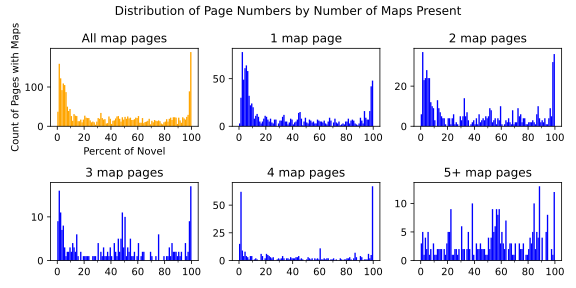
\includegraphics[width=\textwidth]{images/FINAL_page_distr.png}
    \caption{Distribution of page numbers with maps for each page number, after normalizing each novel to 100 pages (i.e., ``1 page'' here  refers to a 1\% chunk of the novel). Each plot contains only novels with exactly $n$ map pages. Maps occur most frequently in the front matter and endpapers, though many occur in the middle for novels with exactly 3 maps.}
    \label{fig:page-num-breakdown}
\end{figure}

By normalizing each novel to 1\% chunks, the distribution of map pages can be compared across novels. Figure \ref{fig:page-num-breakdown} shows that these maps are not distributed evenly: most maps occur on endpapers (chunks 2, 3, 98, 99) or front matter (chunks 4-10). As endpapers are often a 2-page spread, these novels will almost always have 4 map pages in them.\footnote{Library ownership or checkout information is often pasted into the inside back cover, which could cover the map sufficiently that the classifiers miss it. Theoretically, there are always 4 maps on the endpapers if there is even 1 on the endpapers, even if the data in this dataset does not always reflect that.} Novels with 1 or 2 map pages follow the general trend of all pages with more of these map pages focused in the endpapers and front matter. Novels with 3 map pages have a cluster of these pages occurring in the middle of the novel. This could reflect the actual construction of the novel, as plate sections are often in the middle of a book. Novels with 4 map pages have very few maps in the middle pages, indicative that all 4 maps appear on the endpapers exclusively. Novels with more than 4 map pages appear to distribute those pages randomly throughout the novel.

\subsection{Frequency over Time}
The distribution of map novels over time peaks in 1901, supporting Bushell's claim. The rise in map novels begins in the late 19th century, then tapers off approaching the public domain cutoff of 1928, though this may be an artifact of the public domain limitations of this dataset. Figure \ref{fig:illustr_graphs} shows the number of volumes published per year and the number of maps published per year.

However, there was also a general increase in publications in this dataset at the same time. Figure \ref{fig:freq_perc} shows what percentage of novels are map novels per year. Generally, the increase in map novels outpaces the increase of all novels at the turn of the 20th century. The invention and easier access to lithography could explain the increase in maps toward the end of the 19th century. An analysis of contemporary map novels would provide more insight into how technology might affect the frequency of map novels with the advent of GIS and other digital technologies.

\begin{wrapfigure}{r}{0.5\textwidth}
    \centering
    %\includesvg[width=\linewidth]{images/FINAL_map_year_vol.svg}
    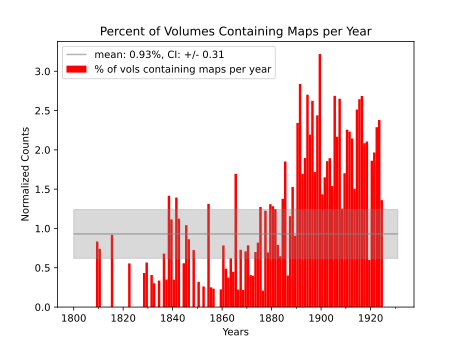
\includegraphics[width=\linewidth]{images/FINAL_map_year_vol.png}
    \caption{Percent of volumes published with maps per year 1800--1925. The annual mean is 0.93\%.}
    \label{fig:freq_perc}
\end{wrapfigure}

\subsection{Metadata}
While MARC metadata for the presence of maps is not reliable for our corpus, metadata in general provides useful context for map novels. The author with the most map novels is G.{\thinspace}A.\ Henty, who wrote primarily historical fiction for young adults. The maps in his novels tend to show scenes of battles from specific historical events. Other top authors include Thomas Hardy, Robert Louis Stevenson, Mark Twain, Rudyard Kipling, Jonathan Swift, Walter Scott, Daniel Defoe, Anna Katherine Green, and John R.\ Musick.

Robert Louis Stevenson was third on the list, even though his only map was of Treasure Island. Henty and Hardy have a greater number of unique stories, with Hardy often reusing the same map of Wessex and Henty generally having a unique map for each novel. Harper \& Brothers and Charles Scribner's Sons were the two most common publishers of map novels in this corpus, despite G.{\thinspace}A.\ Henty publishing with Blackie \& Son.

\subsection{Fictionality \& Scale}
We next consider whether maps are more likely to represent fictional or real places. On one hand, a fictional setting may require a reader to track characters in relation to points of interest that do not align with reality. Such a map would thus serve as a tool for the reader to track the progress of the story. Under this ``Tolkien hypothesis,'' greater unreality produces a greater need for a map. 

Another line of reasoning -- the ``Henty hypothesis'' -- suggests that stories with real settings may contain spatial detail beyond what the reader has as background knowledge. A map of a very small area or a map showing precise movements of soldiers in a battle might require such precision that an average reader could not possibly know this information in advance or track it during extended narration. Thus, highly realistic stories should necessitate a greater need for maps.

Both of these hypotheses presuppose an intent from the author to assist the reader in understanding the spatial content of a story. A null hypothesis would be that authors write their stories with no consideration for spatial navigation.

In our collection, fictional maps make up just 24.8\% of maps in the dataset. 
While fully resolving the Tolkien/Henty hypotheses would require knowledge of the base frequency of real and imaginary settings in novels, we can say that fictional places are less represented in maps overall.
Henty's maps often depict a specific moment in time, one that the average reader may not have sufficient contextual information to follow (in this case, specific movements of troops in battle). Some maps may be of a small enough scale or remote enough location that readers again may lack the baseline knowledge to follow the story.

\begin{table}[htb]
\centering
\begin{tabular}{ l|rr|r }
%\centering
 %\hline
  & Fictional & Real & Total\\
 \hline
 Small Scale & 4.42\% & 3.59\% & 8.01\% \\
 Medium Scale & 3.97\% & 17.12\% & 21.09\% \\
 Large Scale & 16.44\% & 54.46\% & 70.90\% \\ 
 \hline
 Total & 24.83\% & 75.17\% & \\
\end{tabular}
\caption{\label{tab:fict-scale}Fictional maps appear infrequently at the medium scale, while real maps become increasingly represented as the scale becomes larger.}
  \label{fig:illustr_graphs}
\end{table}

Overall, we found that most (70.9\%) maps were of the largest scale. Medium-scale maps make up 21.1\% of the total and small-scale maps, 8.0\%. This does not support the Henty hypothesis, as we would expect readers to be more familiar with larger areas, such as countries or continents, than very small areas, like a specific city or household. If unfamiliarity explained the need for a map, then there would not be any maps of larger areas of real places. This suggests that maps have some other purpose than to be assistive to readers. Table \ref{tab:fict-scale} shows the breakdown of scale and fiction among all maps. Although small-scale maps are uncommon regardless of fictionality, medium-scale maps are much more likely to be of real places than fictional places. Fictional maps mostly depict large areas.

Although there was no genre information included in the MARC records, qualitative analysis suggests that small-scale maps often were in the detective/mystery genre and many of the military history (i.e., Henty) maps were medium scale. We also noticed that many of the fictional maps contained most or all of the typical cartographic features required for a map, such as a legend, scale bar, title, and compass. Many of the real maps lacked some, or even all of these qualities. This could be due to reader familiarity with real places, in which case the author just chooses to include cartographic features that emphasize a certain aspect of spatial distribution.


\subsection{Illustrations}
We found that illustrations were much more common than maps and followed a similar trend of increasing frequency in the late 19th century. However, they decreased in frequency, unlike maps, in the beginning of the 20th century approaching the public domain cutoff. This finding suggests that the trend in map frequency does not follow the overall trend in illustration frequency, which means maps were used fundamentally differently than were illustrations, regardless of whether it was the author or publisher choosing to include the map. Figure \ref{fig:illustr_graphs} shows the prevalence of maps and illustrations.

\begin{figure}
    \centering
    %\includesvg[width=\linewidth]{images/FINAL_illustration_stats.svg}
    \includesvg[width=\linewidth]{images/FINAL_illustration_stats.svg}
    \caption{Frequency of illustrations compared to maps and all novels (left) and the counts of map novels and illustration novels normalized by total novels published per year (right).}
  \label{tab:sp_lang}
\end{figure}


\subsection{Maps and Text}
A reasonable hypothesis is that the text within map novels (i.e., novels that contain at least 1 map) is more spatial than non-map novels. To test this, we used SVM and Naive Bayes algorithms with default \texttt{sklearn} parameters to classify sparse token representations of the 1,557 map novels and an equal number of non-map novels as map-containing or not. SVM achieved an accuracy of 0.81 and Naive Bayes achieved an accuracy of 0.85. These results suggests that there is a relationship between the types of language used in a novel and whether a map is present.

The results of SVM and Naive Bayes classification experiments suggest that there are relationships that exist between the text and the presence of a map. This in turn suggests that authors use fundamentally different language in their novels when those texts contain a map for the reader to reference. However, it is not clear that this difference is due to a focus on the geospatial content of the map. To address this, we finetuned a RoBERTa-based classifier for two tasks: named entity recognition (NER) and geospatial preposition identification. We used the LitBank annotations dataset from Bamman et al.~\cite{bamman2019litbank} for NER finetuning, and geospatial preposition data provided by Radke et al~\cite{radke2022disambiguating}. We also used string matching to identify cartographic features,  including cardinal directions and references to latitude, longitude, altitude, and elevation. In total, there are four spatial categories of interest: geospatial prepositions (S-PREP), generic locations (LOC), geopolitical entities (GPE), and cartographic features (CARD). We also collected five non-spatial categories: regular prepositions (N-PREP), facilities (FAC), organizations (ORG), persons (PER), and vehicles (VEH). We identified these features for all map novels and an equal sized sample of non-map novels.

We counted the number of each entity type per 10,000 tokens for each novel, then calculated the Cohen's $d$ statistic for the map novels and non-map novels. We found that the four spatial entities, along with vehicles, appeared more frequently in novels with maps than non-map novels, all with medium to large effect sizes (see table \ref{tab:sp_lang}). We also found that spatial entities appeared almost twice as often in map novels than in non-map novels, while non-spatial terms appeared in similar frequency in both types of novels. These findings suggest that authors use more spatial language when they have maps, which supports the hypothesis that authors are using the maps as a reference source for orienting the reader within the space of the novel.

\begin{table}[htb]
\centering
\begin{tabular}{ l|rrr }
%\centering
 %\hline
 Entity & Map novel mean & Non-map novel mean & Cohen's $d$ \\
 \hline
 \hline
 S-PREP & 194.75 & 141.81 & 0.917 \\
 LOC & 72.00 & 39.45 & 0.814 \\ 
 GPE & 48.75 & 31.44 & 0.630 \\
 CARD & 8.43 & 4.21 & 0.622 \\ 
 \hline
 VEH & 18.38 & 9.41 & 0.601 \\ 
 ORG & 4.10 & 3.62 & 0.155 \\ 
 FAC & 69.79 & 67.24 & 0.086 \\ 
 N-PREP & 961.83 & 969.45 & -0.052 \\ 
 PER & 447.46 & 467.08 & -0.174 \\ 
\end{tabular}
\caption{Frequency of each entity per 10,000 words in map novels and non-map novels. CARD, GPE, LOC, and S-PREP represent the spatial entities of interest, which occur more frequently in map novels than non-map novels.}
  \label{appdx:first}
\end{table}

\section{Conclusion, Limitations, and Future Work}
This paper fills a gap in computational literary cartography by creating a dataset that is geographically broad and lays the groundwork for multimodal approaches by identifying maps alongside their text. Initial analyses suggest that maps 1) are exceedingly rare within fiction, 2) were most popular at the turn of the 20th century, 3) appear most often on endpapers or front matter, 4) are not often captured in MARC records, 5) tend to depict real settings in preference to fictional ones, 6) tend to depict areas at the scale of a region or country, and 7) appear in novels that have text distinct from that of novels without maps.

Although we generalize our results, our dataset is limited -- as all academic libraries like HathiTrust are -- to being a sample of literature. The dataset is also limited to English volumes, which have not been validated over time or across genres. Likewise the classifiers we created are not perfect, just very good approximations.
This project was also limited by copyright considerations to volumes published before 1928. Extending this work to the present day would be a natural and valuable next step. Contemporary conceptions of literary maps are strongly influenced by fantasy maps, such as those in Tolkien's \emph{The Lord of the Rings}, a famous example of maps in novels.
We were surprised to find that public domain maps were mostly of real places rather than fictional ones, and that many maps seemed to be in historical fiction novels.

This work can add to our ability to study spatial content in literature. Computational approaches to analyzing the geospatial content of novels have to date relied on what can be extracted from the text directly~\cite{wilkens2024small,soni2023grounding}, focusing on fictional stories with real settings. However, the inclusion of fictional maps in some novels provides a geospatial ground-truth that contextualizes the exact places that are the focus of that novel. 

Analyzing an author's intention to include a map in their novel implies that they want to influence readers in some way with this map. Perhaps authors use more spatial language to direct the readers to the map or they offload all spatial information onto the map and the text includes very little spatial language. Performing more thorough analysis on the relationship between maps and the text content of the novel will provide further insight into our initial finding that the two seem to be related. Likewise, the behaviors of readers can be similarly examined between novels with maps and those without to see whether the presence of a map influences how readers think about the spaces within a novel. Do readers even reference these maps as they read? Text analysis to see what kind of language authors use in their novels and readers use in their reviews can reveal whether maps get people to think about novels in a more spatial way.


\section*{Acknowledgments}

We thank Alina Shah for assisting with data annotation tasks. We also thank Federica Bologna, Anna Choi, Sil Hamilton, Rebecca Hicke, Kiara Liu, Sanghoon Oh, Andrew Piper, Rosamond Thalken, Andrea Wang, and Shengqi Zhu for their feedback and support. This project was supported in part by the National Endowment for the Humanities (\#HAA-290374-23, ``AI for Humanists,'' to MW and DM).

% Print the biblography at the end. Keep this line after the main text of your paper, and before an appendix. 
\printbibliography

% You can include an appendix using the following command
\appendix

\section{CLIP Prompts} 
\hfill\\*\noindent\textbf{Map prompt:} 
\begin{verbatim}
"Maps contain top-down views of cartographic features, 
such as roads, waterways, cities, countries, or floorplans. Maps and 
floorplans could have text on the same page as them or be cropped or 
obscured. Maps may be old, hand-drawn, or artistic. Maps can appear 
anywhere on the page."
\end{verbatim}

\hfill\\*\noindent\textbf{Non-map prompt:} \begin{verbatim}
"Pages that are not maps contain illustrations, photographs, 
landscapes, diagrams, text, front covers, front matter, library stamps, 
or decorative end pages and do not have maps anywhere on the page. 
Pages without maps may have both illustrations and text."
\end{verbatim}

\section{Computational Costs} \label{appdx:second}
We chose our computational methodology based off of the premise that close-reading does not scale to the number of novels that are needed to make conclusions that generalize to all of English language literature. Even with computational methods, processing time can vary between that which can be done on a laptop with only a CPU to projects that require a dedicated server with a GPU to projects that require multiple nodes in a large computational cluster or datacenter. In the effort of reproducibility, we want to provide detail on the compute required for this project.

All computing was done on a server with a single A6000 GPU and the dataset takes up 6.2 TB of storage. Code was optimized to use the GPU when applicable. Each stage of the classification process took different amounts of time, based on the efficiency of the model being used and the number of images that need to be processed. Table \ref{tab:model_costs} shows how long each classification step took and the relative cost to rent an A6000 GPU.

\begin{table}[htb]
\centering
\begin{tabular}{ lr|rrr }
\centering
 Model & Image Size & Images Processed & Time Taken (Hours) & Hypothetical Cost \\
 \hline
 EfficientNet\_b0 & 512 & 32,177,400 & 139 & \$62.55 \\
 EfficientNet\_b7 & 768 & 32,177,400 & 206 & \$92.70 \\
 EfficientNet\_V2\_l & 1024 & 32,177,400 & 236 & \$106.20 \\ 
 CLIP & 224 & 584,143 & 7 & \$3.15 \\
 Human Annotation & full size & 15,298 & 8 & \$124.00 \\
\end{tabular}
\caption{Computational and time costs of each step in the classification process, using an A6000 GPU. Costs for the models are assuming \$0.45/hour and \$15.50 for the human annotators (New York State minimum wage).}
\label{tab:model_costs}
\end{table}

%Appendix sections should be ordered by letters rather than numbers, and their contents do not count towards the paper's length limit. Appendix sections may also contain additional tables and figures.  

\end{document}
